\chapter{三维空间刚体运动}

\section{旋转矩阵} 

\subsection{点和向量,坐标系}

    如何表示一个点在三维空间,假设一个线性空间的基为:$(e_1, e_2, e_3)$,那么:

$$
a = 
\begin{bmatrix}
e_1, & e_2, & e_3
\end{bmatrix}
\begin{bmatrix}
a_1 \\
a_2 \\
a_3 
\end{bmatrix} = a_1e_1 + a_2e_2 + a_3e_3
$$

    对于向量的内积:

$$
    a \cdot b = a^Tb = \sum_{i = 1}^3{a_ib_i} = |a||b|cos<a, b>
$$

    对于向量的外积:

$$
a \times b = 
\begin{bmatrix}
i & j & k \\
a_1 & a_2 & a_3 \\
b_1 & b_2 & b_3 
\end{bmatrix} = 
\begin{bmatrix}
a_2b_3 - a_3b_2 \\
a_3b_1 - a_1b_3 \\
a_1b_2 - a_2b_1
\end{bmatrix} = 
\begin{bmatrix}
0 & -a_3 & a_2 \\
a_3 & 0 & -a_1 \\
-a_2 & a_1 & 0
\end{bmatrix}b \triangleq a^\land b
$$

    外积的方向垂直于这两个方向,大小为$|a||b|sin<a, b>$。对于外积,此处引入了${}^\land$符号,把$a$携程一个矩阵。事实上是一个反对称矩阵($Skew-symmetric$),可以将${}^\land$记成一个反对称符号。

    外积只对三维向量存在定义,可以用外积表示向量的旋转

\subsection{坐标系间的欧式变换}

\begin{quote}
    \centering
    描述两个坐标系之间的旋转关系,加上平移统称为坐标系之间的变换关系
\end{quote}

\begin{figure}[!htbp]
    \centering
    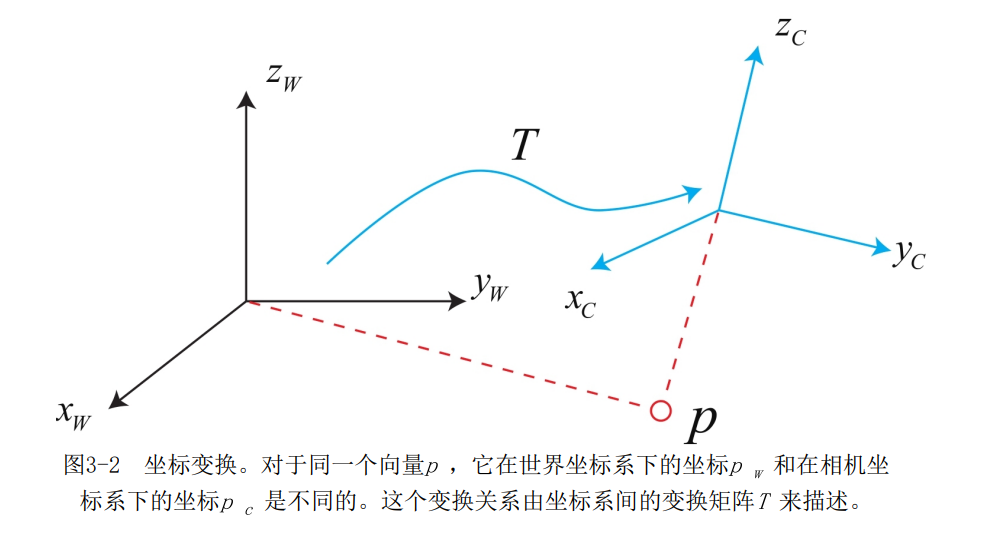
\includegraphics[width=0.3\textwidth]{image/chapter02/坐标系的旋转.png}
    \caption{坐标系的旋转}
\end{figure}

    \emph{相机运动是一个刚体运动,保证了同一个向量再各个坐标系下的长度和角度不会发生变化},这被称为欧式变换。

    一个欧式变换由\emph{一个旋转和一个平移两部分组成}。首先考虑旋转,我们设某个单位正交基$(e_1, e_2, e_3)$经过一次旋转变为$(e_1^{'}, e_2^{'}, e_3^{'})$,那么对于同一个向量$a$(\emph{该向量并没有随着坐标系的旋转而发生运动}),它再这两个坐标系下的坐标分别为:$\begin{bmatrix}a_1, & a_2, & a_3\end{bmatrix}^T$和$\begin{bmatrix}a_1^{'}, & a_2^{'}, & a_3^{'}\end{bmatrix}^T$,那么就有:

$$
\begin{bmatrix}
    e_1, & e_2, & e_3
\end{bmatrix}
\begin{bmatrix}
    a_1 \\ a_2 \\ a_3
\end{bmatrix} = 
\begin{bmatrix}
    e_1^{'}, & e_2^{'}, & e_3^{'}
\end{bmatrix}
\begin{bmatrix}
    a_1^{'} \\ a_2^{'} \\ a_3^{'}
\end{bmatrix}
$$

    此时将上述等式的左右两边同时乘上$\begin{bmatrix}e_1^{T} \\ e_2^{T} \\ e_3^{T}\end{bmatrix}$:

$$
\begin{bmatrix}
    a_1 \\ a_2 \\ a_3
\end{bmatrix} = 
\begin{bmatrix}
    e_1^Te_1^{'}, & e_1^Te_2^{'}, & e_1^Te_3^{'} \\
    e_2^Te_1^{'}, & e_2^Te_2^{'}, & e_2^Te_3^{'} \\
    e_3^Te_1^{'}, & e_3^Te_2^{'}, & e_3^Te_3^{'} 
\end{bmatrix}
\begin{bmatrix}
    a_1^{'} \\ a_2^{'} \\ a_3^{'}
\end{bmatrix} \triangleq Ra^{'}
$$

    我们把中间的矩阵拿出来,定义成一个矩阵$R$。\emph{这个矩阵由两组基之间的内积组成,刻画了旋转前后同一个向量的坐标变换关系}。只要旋转是一样的,这个矩阵也是一样的。\emph{可以说,矩阵$R$描述了旋转本身,因此又称为旋转矩阵}

    旋转矩阵本身有一些特别的性质,比如它是一个行列式为1的正交矩阵,反之,行列式为1的正交矩阵也是一个旋转矩阵。因此,可以定义:

$$
	SO(n) = \{R \in \mathbb{R}^{n \times n} | RR^T = I, det(R) = 1 \}
$$

    $SO(n)$是特殊正交群($Special Orthogonal Group$)的意思(下一讲)。\emph{旋转矩阵可以描述相机的旋转},而$R$满足以下性质:


$$
\begin{aligned}
	a^{'} &= R^{-1}a = R^Ta \\
	a_1 &= R_{12}a_2 \\
	a_3 &= R_{32}a_2 = R_{32}R_{21}a_1 = R_{31}a_1
\end{aligned}
$$

    最后考虑世界坐标系中的向量$a$经过一次旋转和一次平移$t$后,得到$a^{'}$:

$$
    a^{'} = Ra + t
$$

    其中,$t$被称为平移向量,相比于旋转,平移部分只需要把这个平移量加到旋转后的坐标上。

\subsection{变换矩阵与齐次坐标}

    假定在上述给出的式子上我们进行了两次变换:$R_1,t_1$和$R_2,t_2$:

$$
    b = R_1a + t_1 ,\quad c = R_2b + t_2
$$

    那么就能够得到从$a$到$c$的变换:

$$
    c = R_2(R_1a + t_1) + t_2
$$

    这样的形式在多次变换后会很复杂,因此引入齐次坐标和变换矩阵重写:

$$
\begin{bmatrix}
    a^{'} \\ 1
\end{bmatrix} = 
\begin{bmatrix}
    R & t \\ 
    0^T & 1
\end{bmatrix}
\begin{bmatrix}
    a \\ 1
\end{bmatrix} \triangleq T 
\begin{bmatrix}
    a \\ 1
\end{bmatrix}
$$

    用这四个坐标表示三维向量的做法称为齐次坐标,引入齐次坐标后,旋转和平移可以放入同一个矩阵,称为变换矩阵,记作$T$矩阵。那么,经过多次变换后,通过变换矩阵可以得出:

$$
    \tilde{b} = T_1\tilde{a}, \tilde{c} = T_2\tilde{b} \Rightarrow \tilde{c} = T_2T_1\tilde{a}
$$

    对于变换矩阵,具有比较特别的结构:左上角为旋转看矩阵,右侧为平移向量,左下角为零向量,右下角为1。这种矩阵又称为特殊欧式群($Special Euclidean Group$)

$$
se(3) = \{ T = 
\begin{bmatrix}
    R & t \\
    0^T & 1
\end{bmatrix} \in \mathbb{R}^{4 \times 4} | R \in SO(3), t \in \mathbb{R}^3
\}
$$

    那么可以因此求得该矩阵的一个反向的变换:

$$
T^{-1} = 
\begin{bmatrix}
    R^T & -R^Tt \\
    0^T & 1
\end{bmatrix}
$$

\subsubsection{例子}

\begin{quote}
    \centering
    在Slam中,通常定义世界坐标系$T_W$与机器人坐标系$T_R$
\end{quote}

    一个点的世界坐标系为$p_W$,机器人坐标系下为$p_R$,则有:$p_R = T_{RW}p_W$。 也就是说,机器坐标系的点$p_R$可以由世界坐标系下的点$p_W$通过$T_{RW}$变换得到

\section{Eigen}

    对于Eigen的安装来说,这是一件非常容易的事(指在Linux操作系统或类Unix操作系统上),我们只需要键入以下命令:

\begin{lstlisting}[language=C++]
    sudo apt-get install libeigen3.dev
\end{lstlisting}

    对于Eigen第三方库的使用来说,也是较为简便的,因为Eigen只有头文件,是的,因此我们可以在\emph{CMakeLists.txt}文件中使用以下条件命令来引入:

\begin{lstlisting}[language=C++]
    find_package(Eigen3 REQUIRED)
    include_directories(${EIGEN3_INCLUDE_DIRS})
\end{lstlisting}

\subsection{Eigen的使用示例}

    对于Eigen来说,其使用是需要了解Eigen库的,此处我们使用一个小的例子来说明如何使用Eigen

\begin{lstlisting}[language=C++]
#include <iostream>
#include <ctime>
#include "eigen3/Eigen/Core"
#include "eigen3/Eigen/Dense"

#define MATRIX_SIZE 50

int main() {
    Eigen::Matrix<float, 2, 3> matrix_23;
    Eigen::Vector3d v_3d;
    Eigen::Matrix3d matrix_33 = Eigen::Matrix3d::Zero();
    Eigen::Matrix<double, Eigen::Dynamic, Eigen::Dynamic> matrix_dynamic;
    Eigen::MatrixXd matrix_x;

    matrix_23 << 1, 2, 3, 4, 5, 6;
    std::cout << matrix_23 << std::endl;

    for (int i = 0; i < 1; i++) {
        for (int j = 0; j < 2; j++)
            std::cout << matrix_23(i, j) << " ";
        std::cout << "\n";
    }

    v_3d << 3, 2, 1;
    // Eigen::Matrix<double, 2, 1> result_wrong_type = matrix_23 * v_3d;
    Eigen::Matrix<double, 2, 1> result = matrix_23.cast<double>() * v_3d;
    std::cout << result << std::endl;

    matrix_33 = Eigen::Matrix3d::Random();
    std::cout << matrix_33 << std::endl;
    std::cout << matrix_33.transpose() << std::endl;
    std::cout << matrix_33.sum() << std::endl;
    std::cout << matrix_33.trace() << std::endl;
    std::cout << 10 * matrix_33 << std::endl;
    std::cout << matrix_33.inverse() << std::endl;
    std::cout << matrix_33.determinant() << std::endl;

    Eigen::SelfAdjointEigenSolver<Eigen::Matrix3d> eigen_solver(matrix_33.transpose() * matrix_33);

    std::cout << "Eigen value: " << eigen_solver.eigenvalues() << std::endl;
    std::cout << "Eigen vectors: " << eigen_solver.eigenvectors() << std::endl;

    Eigen::Matrix<double, MATRIX_SIZE, MATRIX_SIZE> matrix_NN;
    matrix_NN = Eigen::MatrixXd::Random(MATRIX_SIZE, MATRIX_SIZE);
    Eigen::Matrix<double, MATRIX_SIZE, 1> v_Nd;
    v_Nd = Eigen::MatrixXd::Random(MATRIX_SIZE, 1);

    clock_t tiem_stt = clock();
    Eigen::Matrix<double, MATRIX_SIZE, 1> x = matrix_NN.inverse() * v_Nd;
    std::cout << "tiome use in normal invers is: " << 1000 * (clock() - tiem_stt) / (double)CLOCKS_PER_SEC << "ms" << std::endl;

    tiem_stt = clock();
    x = matrix_NN.colPivHouseholderQr().solve(v_Nd);
    std::cout << "tiome use in Qr compsition invers is: ";

    return 0;
\end{lstlisting}

\section{旋转向量和欧拉角}

\subsection{旋转向量}

    我们回到理论部分,探究矩阵表示方式中的缺点:

\begin{itemize}
    \item [1)] $SO(3)$的旋转矩阵由9个量,但一次旋转只有三个自由度,因此是冗余的
    \item [2)] 旋转矩阵自身带有约束:必须是正交矩阵,且行列式为1
\end{itemize}

    我们希望有一种方式能够紧凑的描述旋转和平移,我们知道\emph{任意旋转都可以用一个旋转轴和一个旋转角}来刻画,语句我们使用一个向量,\emph{其方向与旋转轴一致,而长度等于旋转角,这种向量被称为旋转向量(或轴角,$Axis-Angle$)}

$$
    w = \theta{n}
$$

    这是下一节中的李代数,因此目前只需要了解这样表示即可。之后,从旋转向量到旋转矩阵的转换过程由罗德里格斯公式($Rodrigues's Formula$)表明:

$$
    R = cos\theta{I} + (1 - cos\theta)nn^T + sin\theta{n^\land}
$$

    符号$\land$是向量到反对称的转换符,反之,我们也可以有一个旋转矩阵到旋转向量的转换:

$$
\begin{aligned}
    tr(R) &= cos\theta{tyr(I)} + (1 - cos\theta)tr(nn^\land) + sin\theta{tr(n^\land)} \\
        &= 3cos\theta + (1 - cos\theta) \\
        &= 1 + 2cos\theta
\end{aligned} \\
$$

    对于转轴$n$,由于旋转轴上的向量在旋转后不发生改变,说明:

$$
    Rn = n
$$

\subsection{欧拉角}

\begin{quote}
    \centering
    无论是旋转矩阵、旋转向量对于人来说不是很直观,因此,欧拉角使用了\emph{三个分离的转角}
\end{quote}

\begin{figure}[!htbp]
    \centering
    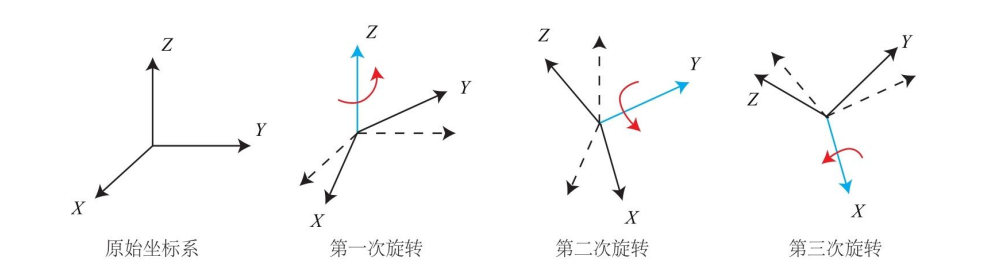
\includegraphics[width=0.6\textwidth]{image/chapter02/欧拉角.png}
    \caption{欧拉角}
\end{figure}

    在欧拉角中,常用的一种是“偏航--俯仰--滚转”($yaw--pitch--roll$)三个角度来描述一个旋转。

\begin{itemize}
    \item [1)] 绕物体的$Z$轴旋转,得到偏航角$yaw$
    \item [2)] 绕物体的$Y$轴旋转,得到俯仰角$pitch$
    \item [3)] 绕物体的$X$轴旋转,得到滚转角$roll$
\end{itemize}
    
\begin{figure}[!htbp]
    \centering
    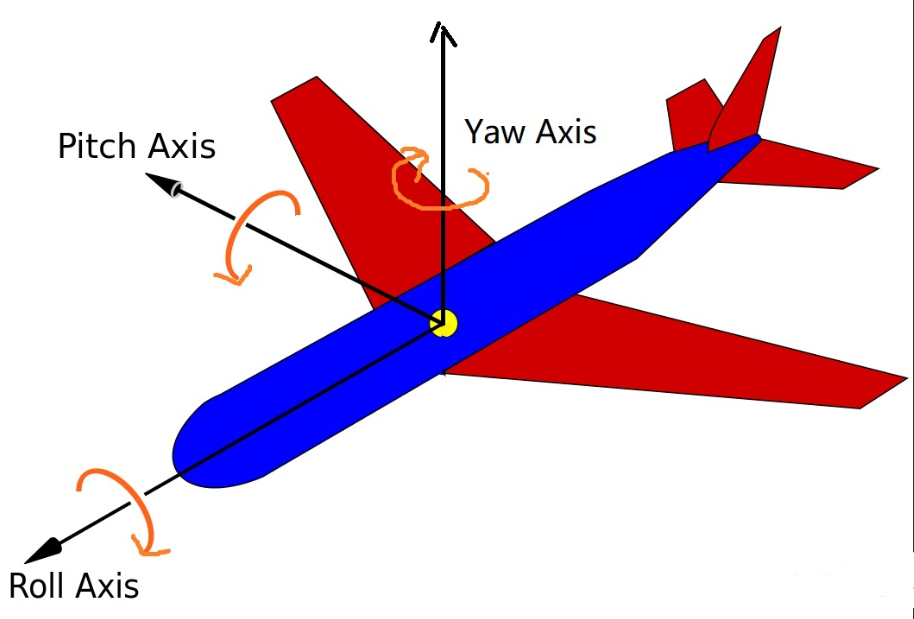
\includegraphics[width=0.4\textwidth]{image/chapter02/ZYX欧拉角.png}
    \caption{Z-Y-X欧拉角}
\end{figure}

    此时,可以使用$\begin{bmatrix}r, & p, & y \end{bmatrix}^T$这样的一个三维向量表示任意旋转。

    但是,\emph{欧拉角的一个重大缺点是会碰见著名的万向锁问题($Gimbal Lock$):在俯仰角为$\pm90^{\circ}$时,第一次旋转与第三次旋转将使用同一个轴,使得系统丢失了一个自由度,这被称为奇异性问题}
    
    由于这种原理,欧拉角不适于插值和迭代,往往只适用于人机交互

\begin{figure}[!htbp]
    \centering
    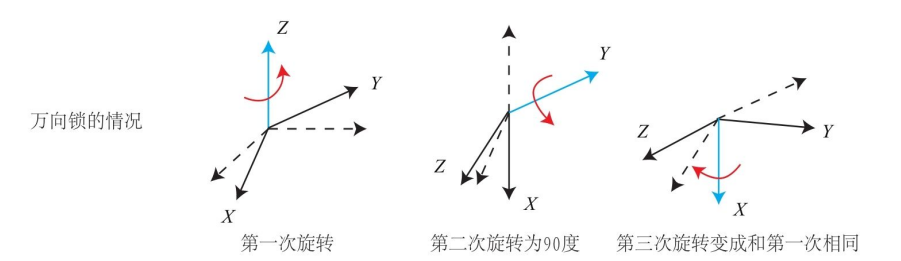
\includegraphics[width=0.6\textwidth]{image/chapter02/万向锁.png}
    \caption{万向锁问题}
\end{figure}

\section{四元数}

\subsection{四元数定义}

    旋转矩阵用9个量描述三个自由度的旋转,但具有冗余性;欧拉角和旋转向量是紧凑的,但具有奇异性。因此,我们需要提出一种新的方式来描述旋转

    回想一下复数:复数的惩罚表示复平面上的旋转。\emph{因此,表达三维空间旋转时,有一种类似复数的代数:四元数($Quaternion$),四元数既是紧凑的,也没有奇异性,唯独不够直观,计算稍微复杂}

    一个四元数$q$拥有一个实部和三个虚部:$q = q_0 + q_1i + q_2j + q_3k$。其中,$i, j, k$为四元数的三个虚部,三个虚部满足:

$$
\begin{cases}
    i^2 = j^2 = k^2 = -1 \\
    ij = k, ji = -k \\
    jk = i, kj = -i \\
    ik = j, ki = -j 
\end{cases}
$$

    我们可以简单的将虚部看作三个转轴向量,但是实际上不是。由于这种特殊的表示形式,我们可以用一个标量和一个向量来表示四元数:

$$
    q = [s, v], s = q_0 \in \mathbb{R}, v = [q_1, q_2, q_3]^T \in \mathbb{R}^3
$$

    这里,$s$称为四元数的实部,$v$称为它的虚部。

\begin{figure}[!htbp]
    \centering
    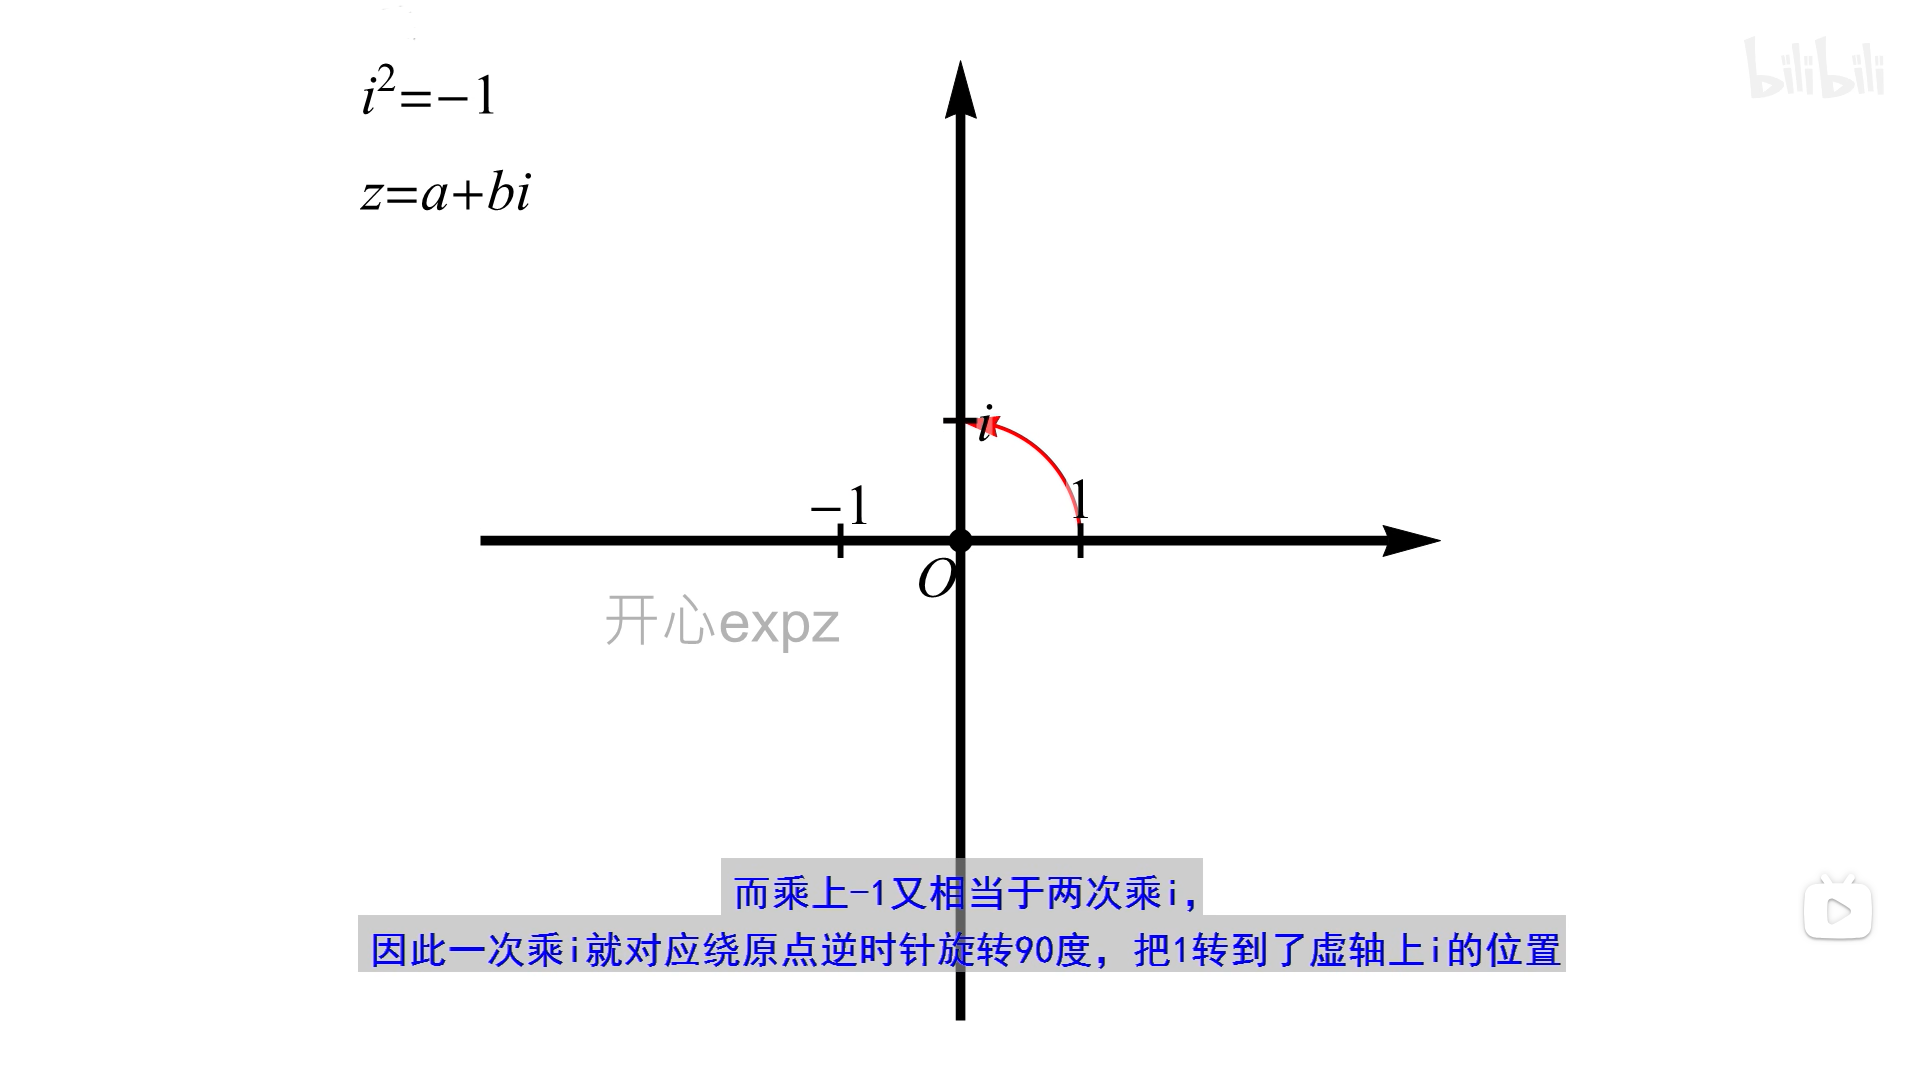
\includegraphics[width=0.5\textwidth]{image/chapter02/二维向量乘法.png}
    \caption{二维向量的乘法}
\end{figure}

    可以看见,从1到-1的过程实际上是旋转了$180^{\circ}$,如果乘以虚数$i$,就相当于绕原点逆时针$90^{\circ}$

\begin{figure}[!htbp]
    \centering
    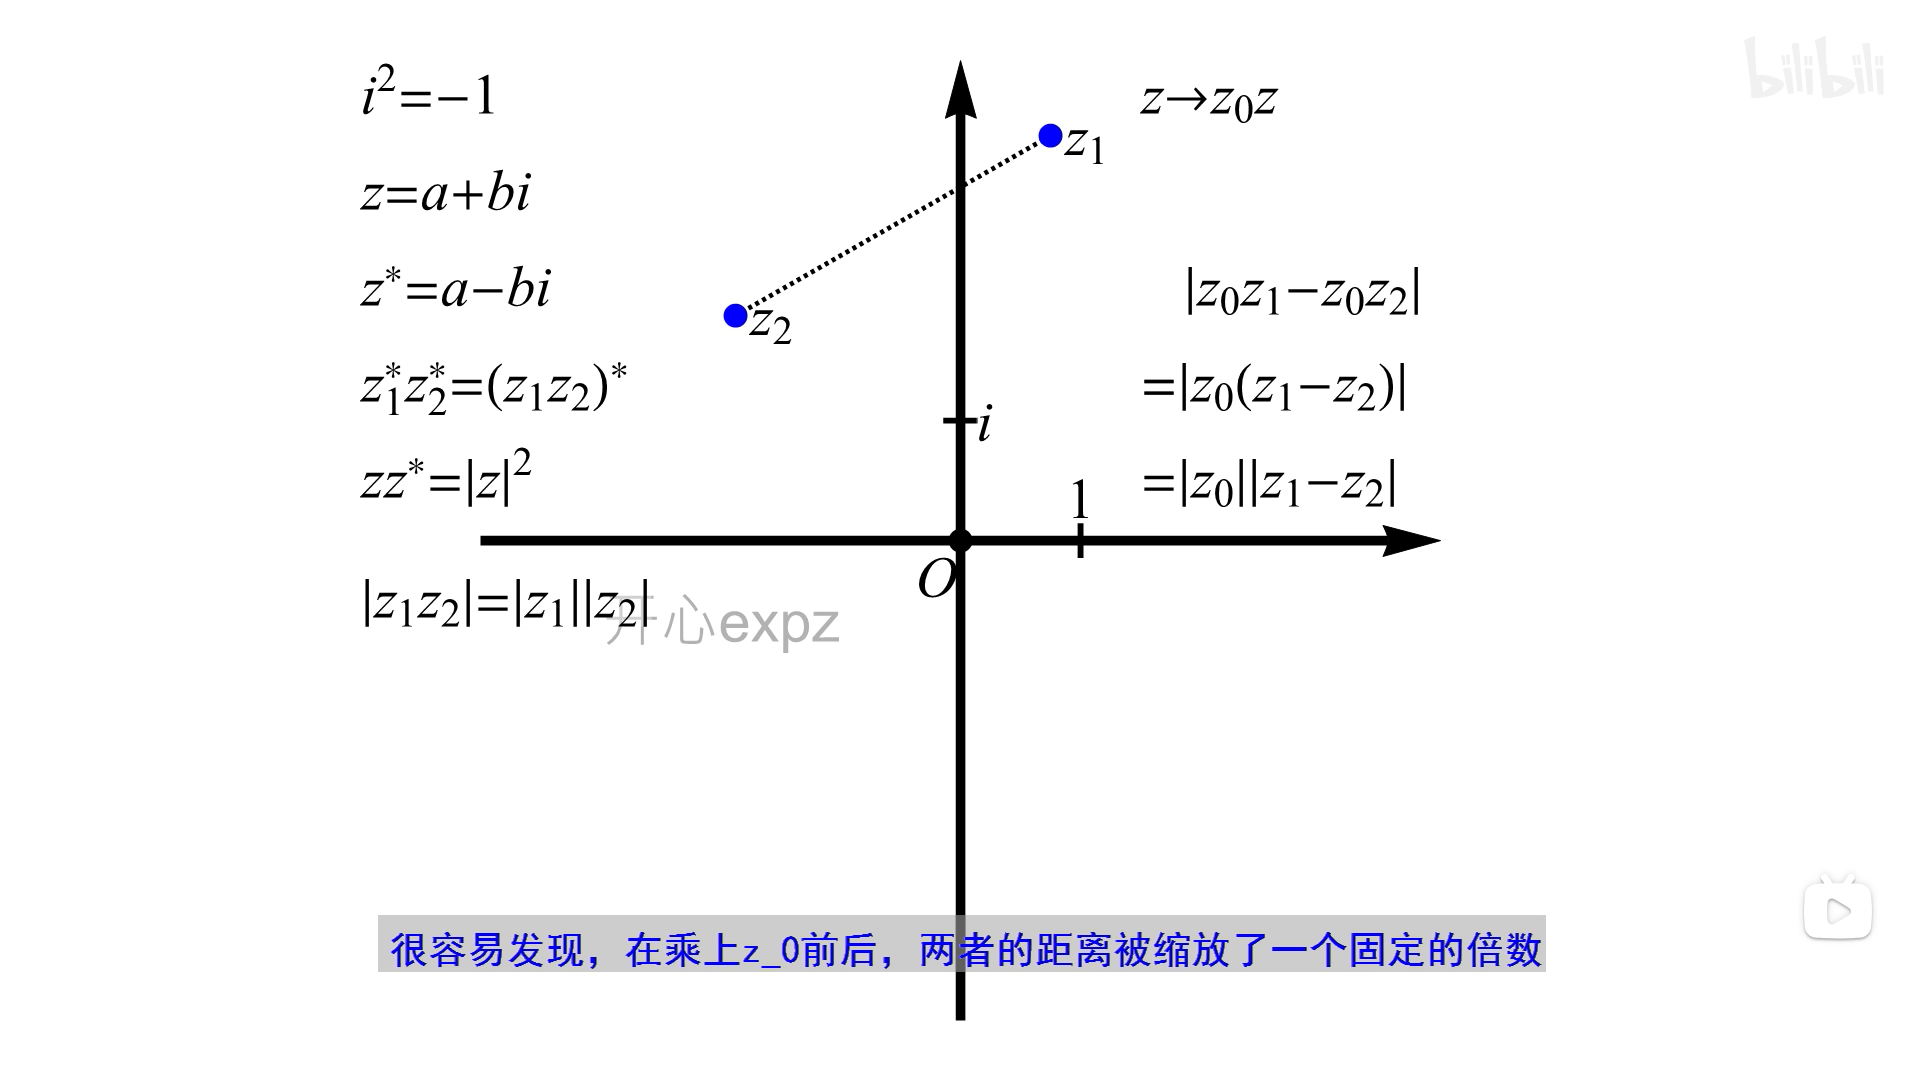
\includegraphics[width=0.6\textwidth]{image/chapter02/二维向量加减.png}
    \caption{二维向量的加法}
\end{figure}

    对于加减,相当于对轴上进行扩张和缩减,对于乘除,就相当于原点不变,进行缩放和扩张以及旋转

\begin{figure}[!htbp]
    \centering
    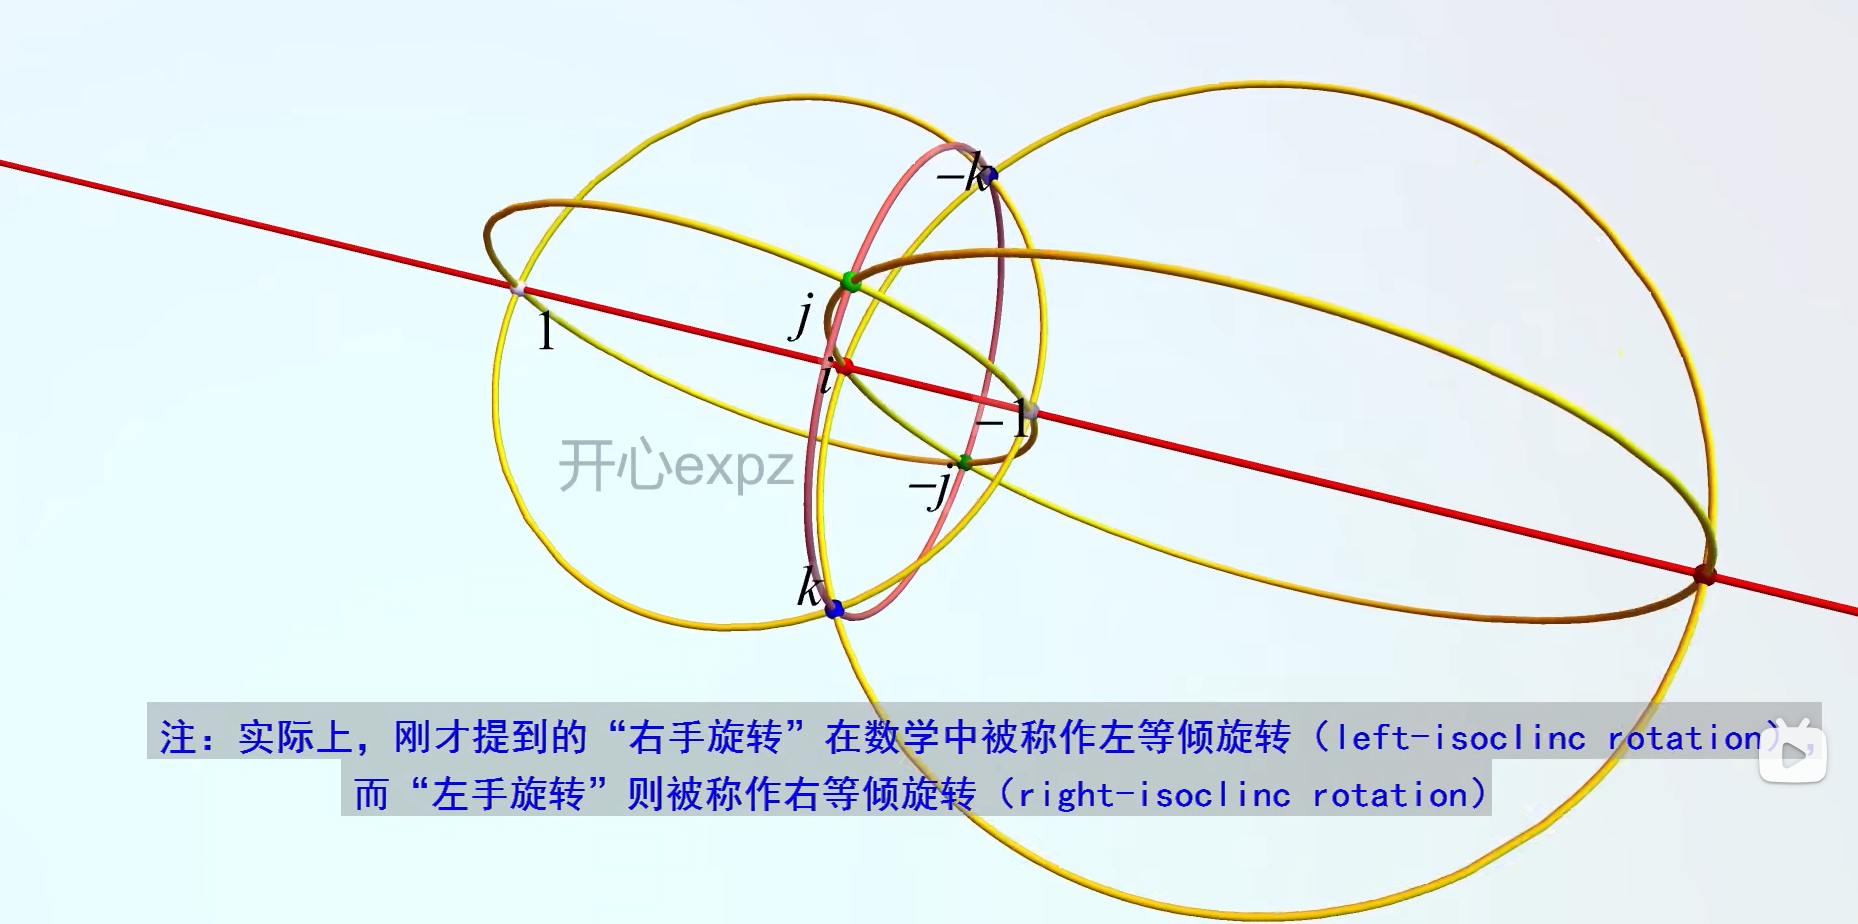
\includegraphics[width=0.6\textwidth]{image/chapter02/四元数到三维的变换模型.png}
    \caption{四元数从四维到三维的变换}
\end{figure}

    因此,对于四元数来说,可以通过四维来表示三维的旋转,$ij = k, ji = -k, i^2 = -1$是必须存在的条件,同时也会随着旋转被映射到无穷远最终回到三维

    同时,我们发现,旋转两个周期才会回到与原先的样子相等。假设某个旋转是绕单位向量$n = [n_x, n_y, n_z]^T$进行了角度为$\theta$的旋转,那么这个旋转可以表示为:

$$
    q = [cos\frac{\theta}{2}, n_xsin\frac{\theta}{2}, n_ysin\frac{\theta}{2}, n_zsin\frac{\theta}{2}]^T
$$

    反之,亦可以得到对应旋转轴与夹角:

$$
\begin{cases}
    \theta = 2arccosq_0 \\
    [n_x, n_y, n_z]^T = [q_1, q_2, q_3]^T / sin\frac{\theta}{2}
\end{cases}
$$

    在四元数中,\emph{任意的旋转都可以由两个互为相反数的四元数表示}。取$\theta$为0,则得到一个没有任何旋转的实四元数:

$$
    q_0 = [\pm1, 0, 0, 0]^T
$$

\subsection{四元数运算}

\begin{quote}
    \centering
    四元数和通常复数一样,可以进行四则运算
\end{quote}

    现有两个四元数$q_a, q_b$,它们的向量表示为$[S_a, V_a],[S_b, V_b]$或者原始四元数$q_a = s_a + x_ai + y_aj + z_ak,q_b = s_b + x_bi + y_bj + z_bk$

\begin{itemize}
    \item 加法减法:$q_a \pm q_b = [S_a \pm S_b, V_a \pm V_b]$
    \item 乘法:
    $$\begin{aligned}
        q_aq_b &= s_as_b - x_ax_b - y_ay_b - z_az_b \\
               &+ (s_ax_b + x_as_b + y_az_b - z_ay_b)i \\
               &+ (s_ay_b - x_az_b + y_as_b + z_ax_b)j \\
               &+ (s_az_b + x_ay_b - y_ax_b + z_as_b)k
    \end{aligned}$$
    \item 使用向量形式并采用内外积运算:$q_aq_b = [s_as_b - v_a^Tv_b, s_av_b + s_bv_a + v_a \times v_b]$
    \item 共轭:$q_a^* = s_a - x_ai - y_aj - z_ak = [s_a, -v_a]$
    \item 模长:$\rVert{q_a}\rVert = \sqrt{s_a^2 + x_a^2 + y_a^2 + z_a^2}$
    \subitem 两个四元数乘积的模即为模的乘积:$\rVert{q_aq_b}\rVert = \rVert{q_a}\rVert \rVert{q_b}\rVert$ 
    \item 逆:$q^{-1} = \frac{q^*}{\rVert{q}\rVert^2}$
    \subitem 四元数与自己逆的乘积为实四元数:$qq^{-1} = q^{-1}q = 1$
    \subitem 如果q为单位四元数,其逆与共轭相等:$(q_aq_b)^{-1} = q_b^{-1}q_a^{-1}$
    \item 数乘:$q_a \cdot q_b = s_as_b + x_ax_bi + y_ay_bj + z_az_bk$
    \item 点乘:$q_a \cdot q_b = s_as_b + x_ax_bi + y_ay_bj + z_az_bk$
\end{itemize}

\subsection{用四元数表示旋转}

    我们可以用四元数表达对一个点的旋转,假设一个空间三维点$p = [x, y, z] \in R^3$,以及一个由轴角$n, \theta$指定的旋转。如果用矩阵旋转描述,那么有$p^{'} = Rp$,那么现在用四元数来表示

    首先将三维空间点用一个虚四元数描述:

$$
    p = [0, x, y, z] = [0, v]
$$

    这相当于将四元数的三个虚部与空间中的三个轴对应,然后:

$$
    q = [cos\frac{\theta}{2}, nsin\frac{\theta}{2}]
$$

    那么经过旋转后的$p^{'}$,可以表示为:

$$
    p^{'} = qpq^{-1}
$$